\subsection{Front-end Implementation}

    The frontend interface layer is developed using React, Vite, TypeScript, and Ant Design. State encapsulation is decoupled across specific user portals to keep operational spaces separate:

    \subsubsection{Admin Console - Create Student Account}

        This screen is used for university admins to create a new student account. It will send an onboard email to the student's email address with the student ID and temporary password for login into the portal.

        \begin{figure}[H]
            \centering
            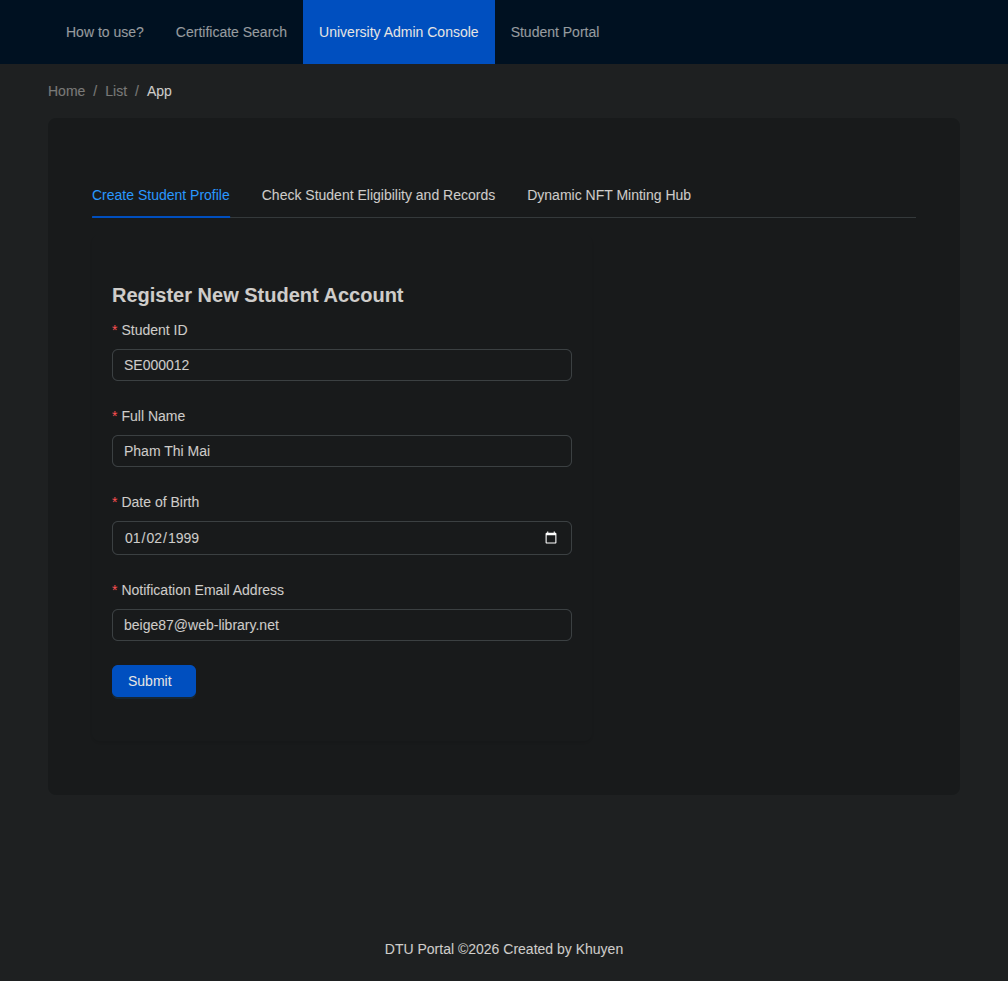
\includegraphics[width=0.85\textwidth, trim=0cm 2cm 0cm 2cm, clip]{images/create_student.png}
            \caption{Admin Console - Add student account}
            \label{fig:create_student}
        \end{figure}

    \subsubsection{Student onboard email}

        \begin{figure}[H]
            \centering
            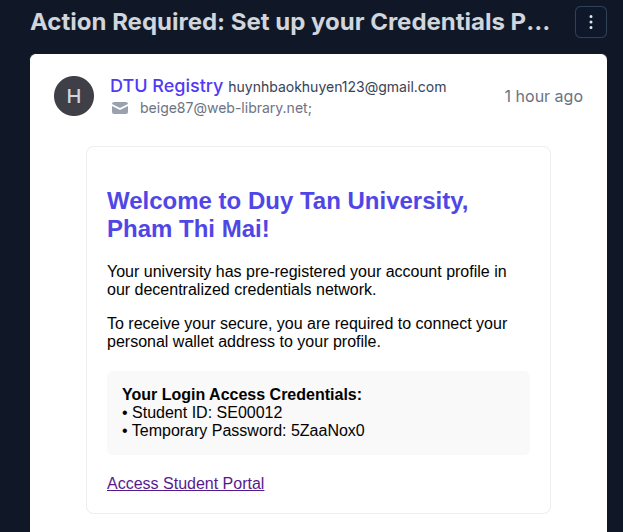
\includegraphics[width=0.85\textwidth, trim=0cm 2cm 0cm 2cm, clip]{images/student_onboard_mail.png}
            \caption{Student onboard email}
            \label{fig:student_onboard_email}
        \end{figure}

    \subsubsection{Student Login}

        This screen used for student login into the portal

        \begin{figure}[H]
            \centering
            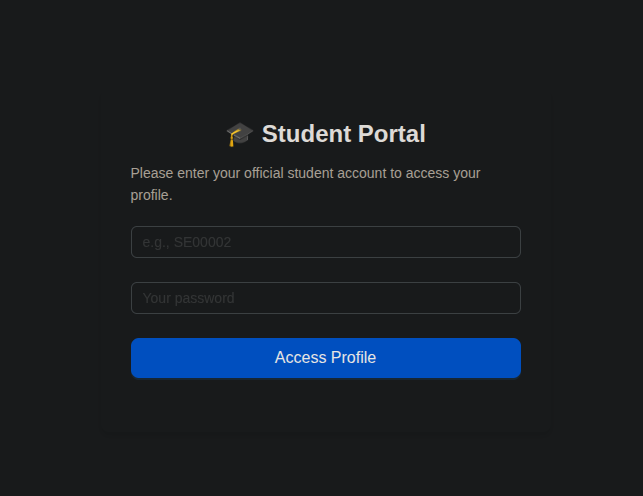
\includegraphics[width=0.85\textwidth, trim=0cm 2cm 0cm 2cm, clip]{images/student_login.png}
            \caption{Student Login}
            \label{fig:student_login}
        \end{figure}

    \subsubsection{Student submits personal wallet address}

        The first time a student logs into the system, they need to submit their wallet address first to save into the system. They can provide a wallet address or connect with the Matemask wallet.

        \begin{figure}[H]
            \centering
            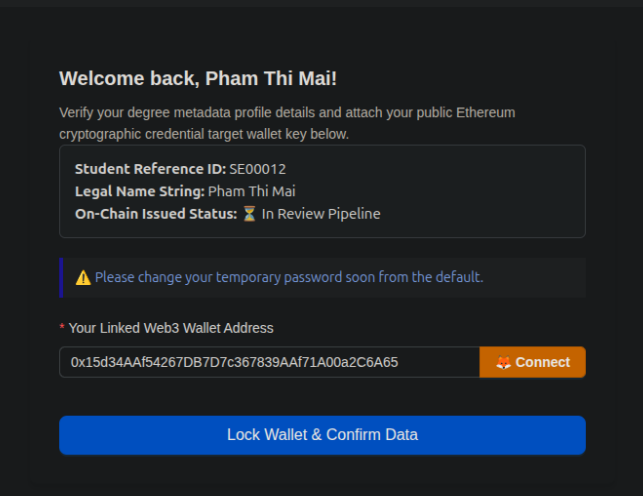
\includegraphics[width=0.85\textwidth, trim=0cm 2cm 0cm 2cm, clip]{images/student_sync_wallet.png}
            \caption{Student Submit Wallet}
            \label{fig:sync_wallet}
        \end{figure}

    \subsubsection{Admin Console - Check for graduation}

        In this screen, the admin can check and see if a student has enough conditions to graduate, and they can create approval for graduation.

        \begin{figure}[H]
            \centering
            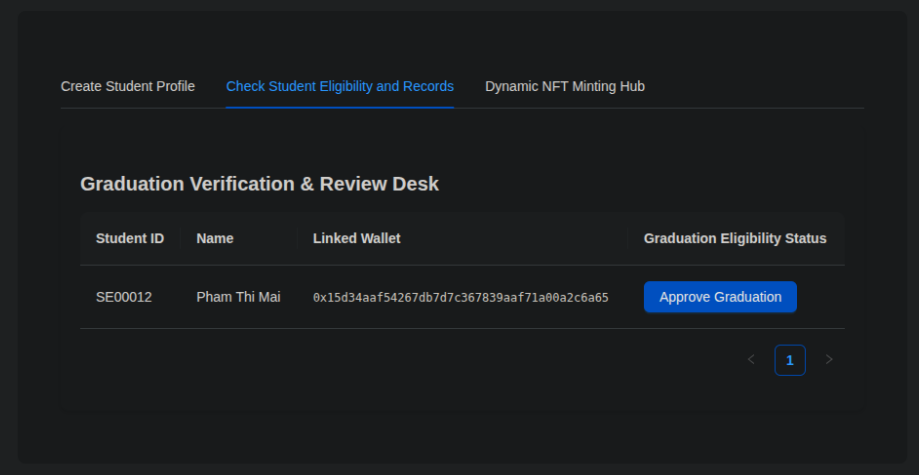
\includegraphics[width=0.85\textwidth, trim=0cm 2cm 0cm 2cm, clip]{images/graduate_approve.png}
            \caption{Admin Console - Graduate Approve}
            \label{fig:graduate_approve}
        \end{figure}

    \subsubsection{Admin Console - Mint graduate certificate}

        After a student is approved for enough conditions to graduate, the admin can mint a certificate. It will connect to the backend api, the backend will process to connect with the IPFS and blockchain side to return the student's PDF certificate file with the hash data.

        \begin{figure}[H]
            \centering
            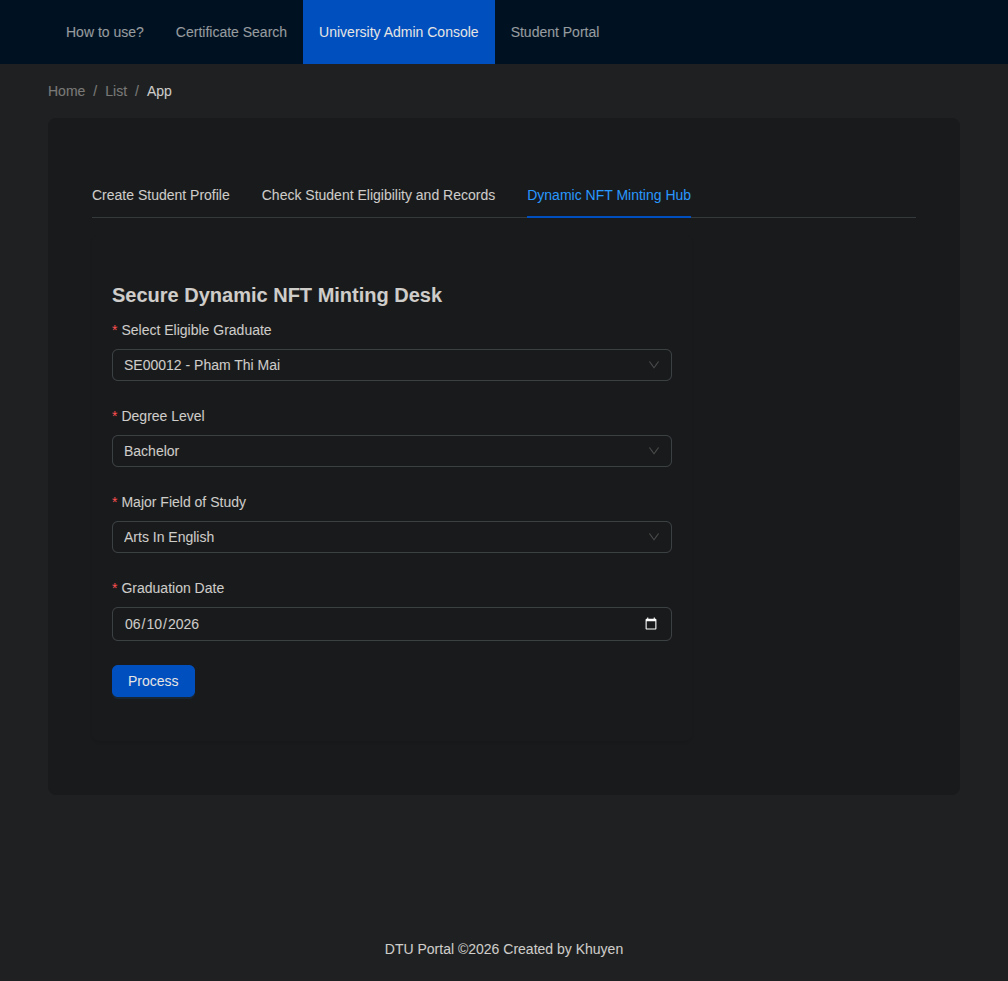
\includegraphics[width=0.85\textwidth, trim=0cm 2cm 0cm 2cm, clip]{images/mint_cert.png}
            \caption{Admin Console - Mint Certificate}
            \label{fig:mint_certificate}
        \end{figure}

        After minting success, the admin can download the PDF certificate file. And an email will auto-send to the student's email with a PDF certificate attached.

        \begin{figure}[H]
            \centering
            
\includegraphics[width=0.85\textwidth]{Degree_Certificate_SE00012.pdf}
            \caption{Admin Console - Mint Certificate - Download Button}
            \label{fig:download_cert}
        \end{figure}

    \subsubsection{Certificate Search}

        This public interface is accessible to all users without requiring authentication. It allows individuals to upload PDF certificates to verify their cryptographic validity against the blockchain registry. Upon processing, the system displays the verification results instantly. Furthermore, the page integrates an AI Agent designed to interpret and explain these cryptographic outcomes in a user-friendly manner

        \begin{figure}[H]
            \centering
            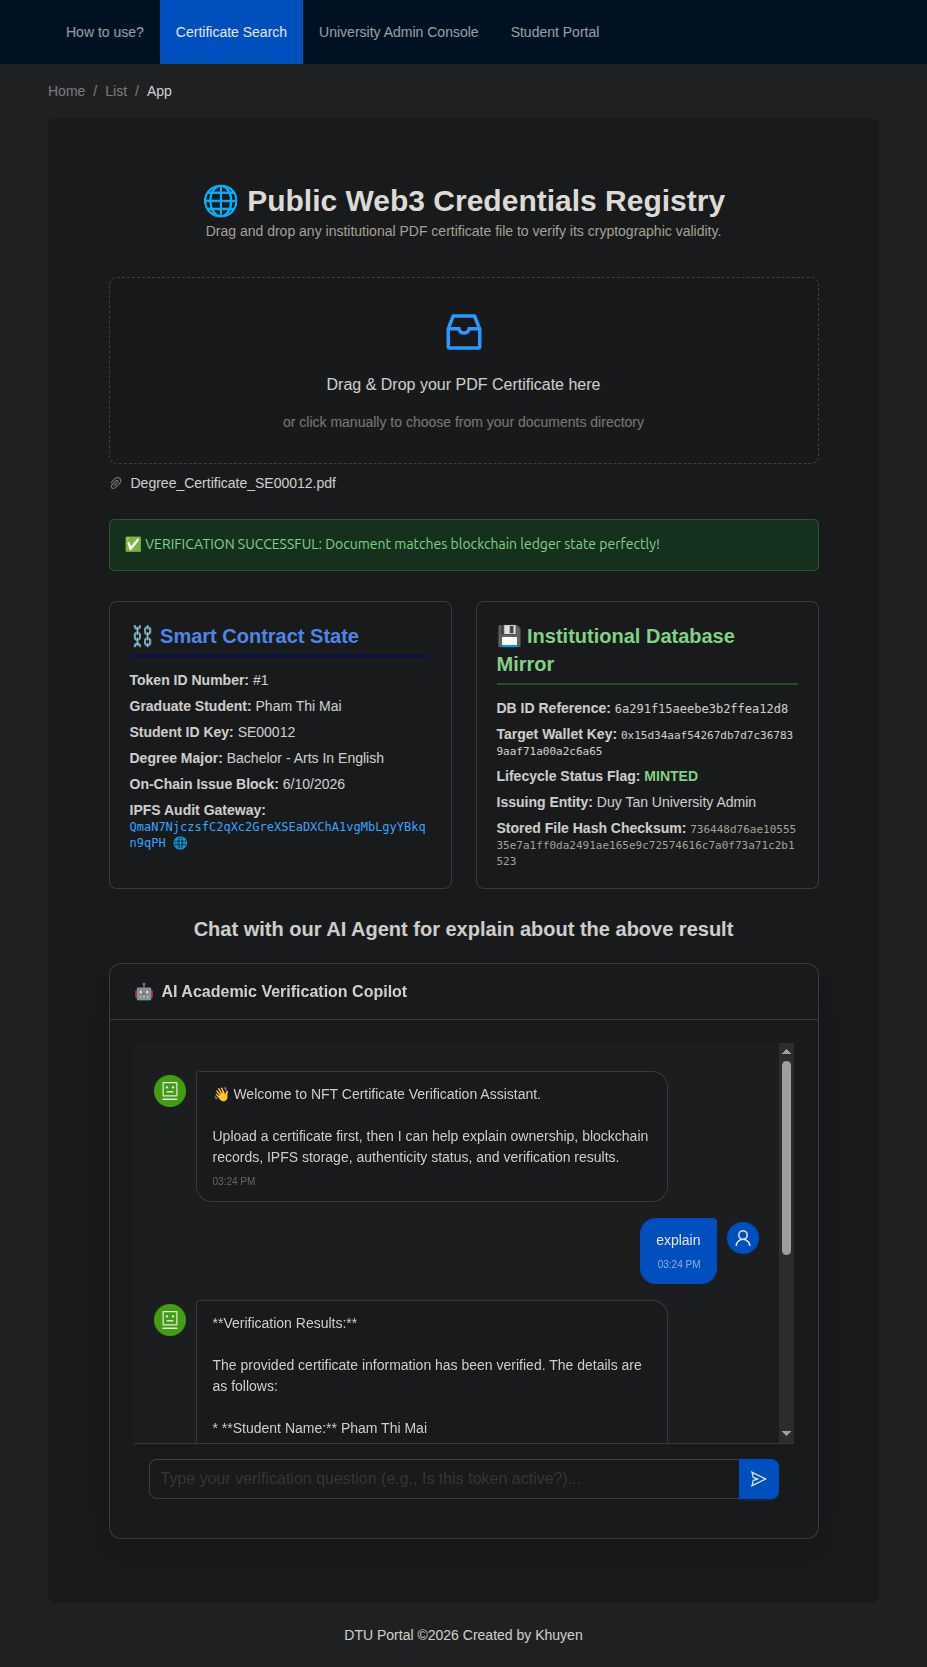
\includegraphics[width=0.85\textwidth, trim=0cm 2cm 0cm 2cm, clip]{images/verify_cert.png}
            \caption{Verify Certificate}
            \label{fig:verify_cert}
        \end{figure}